\documentclass[a4paper]{report}
\usepackage[utf8]{inputenc}
\usepackage[a4paper]{geometry}
\geometry{verbose, marginparwidth=15mm, marginparsep=3mm, tmargin=25mm}
\usepackage[english,ngerman]{babel}
\usepackage[svgnames]{xcolor}
\usepackage{graphicx}
\usepackage[hyphens]{url}
\usepackage[flushmargin,hang]{footmisc}
\usepackage{hyperref}
\usepackage[hypcap]{caption} % link to top of tables and figures, not to bottom caption
\usepackage[parfill]{parskip} % no idented first line of each paragraph
\usepackage{amssymb} % for \checkmark
\usepackage{textgreek} % for \textMu
\usepackage{enumitem} % for \begin{itemize}[label={...}]
\usepackage[export]{adjustbox} % left/right aligned images
\usepackage{float}
\usepackage{tikz}
\usetikzlibrary{arrows,decorations.pathmorphing,backgrounds,fit,positioning,shapes.symbols,chains,shapes.geometric,shapes.arrows,calc}
\usepackage[
backend=biber,
hyperref=true,
url=false,
isbn=false,
backref=false,
% style=custom-numeric-comp,
citereset=chapter,
maxcitenames=3,
maxbibnames=100,
block=none]{biblatex}
\bibliography{sa}
\hypersetup{
	unicode=true,
	pdftitle={Roadster High Availability},
	pdfsubject={Extension of a SCADA Framework to support High Availability and Security},
	pdfauthor={Manuel Schuler, Patrik Wenger},
	pdfkeywords={ruby} {zmq} {czmq} {cztop} {high availability} {security} {encryption} {UPC UA} {SCADA} {C++},
}
\usepackage{csquotes}
\usepackage{pdfpages}
\title{Roadster High Availability}
\author{Manuel Schuler, Patrik Wenger}

\usepackage{MnSymbol}
\usepackage{listings}
\lstloadlanguages{Ruby}
\lstset{language=Ruby}
\lstset{
  prebreak=\raisebox{0ex}[0ex][0ex]{\ensuremath{\hookleftarrow}},
  postbreak=\raisebox{0ex}[0ex][0ex]{\ensuremath{\rcurvearrowse\space}},
}

% custom style for Ruby listings
\lstdefinestyle{customruby}{
  belowcaptionskip=1\baselineskip,
  breaklines=true,
  frame=single,
  frameround=tttt,
  aboveskip=1\bigskipamount,
  belowskip=1\bigskipamount,
  xleftmargin=\parindent,
  language=Ruby,
  showstringspaces=false,
  basicstyle=\footnotesize\ttfamily,
  keywordstyle=\bfseries\color{green!40!black},
  commentstyle=\itshape\color{lightgray!40!black},
  identifierstyle=\color{NavyBlue},
  stringstyle=\color{red},
  captionpos=b,
}

% inline Ruby
% This style can be used within tabular. For some reason, the customruby style
% above won't work. But it has to be used like this (not using the \rb command):
%
% 	\lstinline[style=custominlineruby]{char}
%
\lstdefinestyle{custominlineruby}{
  basicstyle=\ttfamily,
  language=Ruby,
  keywordstyle=\bfseries\color{green!40!black},
  commentstyle=\itshape\color{lightgray!40!black},
  identifierstyle=\color{NavyBlue},
  stringstyle=\color{red},
  breaklines=true,
}

\newcommand{\rb}[1]{\lstinline[
  style=custominlineruby,
  basicstyle=\ttfamily,
  prebreak={},
  postbreak={}]{#1}
}

% custom style for shell command listings
\lstdefinestyle{customsh}{
  language=sh,
  showstringspaces=false,
  basicstyle=\footnotesize\ttfamily,
  breaklines=true,
  frame=single,
  frameround=tttt,
  aboveskip=1\bigskipamount,
  belowskip=1\bigskipamount,
  captionpos=b,
}

% inline shell
\newcommand{\sh}[1]{\lstinline[
  style=customsh,
  basicstyle=\ttfamily,
  prebreak={},
  postbreak={}]{#1}}

\definecolor{diffstart}{named}{Grey}
\definecolor{diffincl}{named}{Green}
\definecolor{diffrem}{named}{OrangeRed}

\usepackage{listings}
\lstdefinelanguage{diff}{
  basicstyle=\ttfamily,
  frame=single,
  frameround=tttt,
  morecomment=[f][\color{diffstart}]{@@},
  morecomment=[f][\color{diffincl}]{+},
  morecomment=[f][\color{diffrem}]{-},
}
\lstdefinestyle{customdiff}{ % custom style for diff command listings
  language=diff,
  showstringspaces=false,
  basicstyle=\scriptsize\ttfamily,
  breaklines=true,
  captionpos=b,
}

\lstdefinelanguage{worddiff}{
  basicstyle=\ttfamily,
  morecomment=[s][\color{diffincl}]{\{+}{+\}},
  morecomment=[s][\color{diffrem}]{[-}{-]}
}
\lstdefinestyle{customworddiff}{ % custom style for git diff --word-diff listings
  language=worddiff,
  showstringspaces=false,
  basicstyle=\scriptsize\ttfamily,
  breaklines=true,
  captionpos=b,
}

\begin{document}
\thispagestyle{empty}
\selectlanguage{english}

% nice looking cover page with help from https://en.wikibooks.org/wiki/LaTeX/Title_Creation
\begin{titlepage}
\centering
\begin{raggedleft}
\includegraphics[trim=10 10 10 10, clip=true, width=0.3\textwidth]{img/hsr_logo.pdf}\end{raggedleft}
\begin{raggedright}\hfill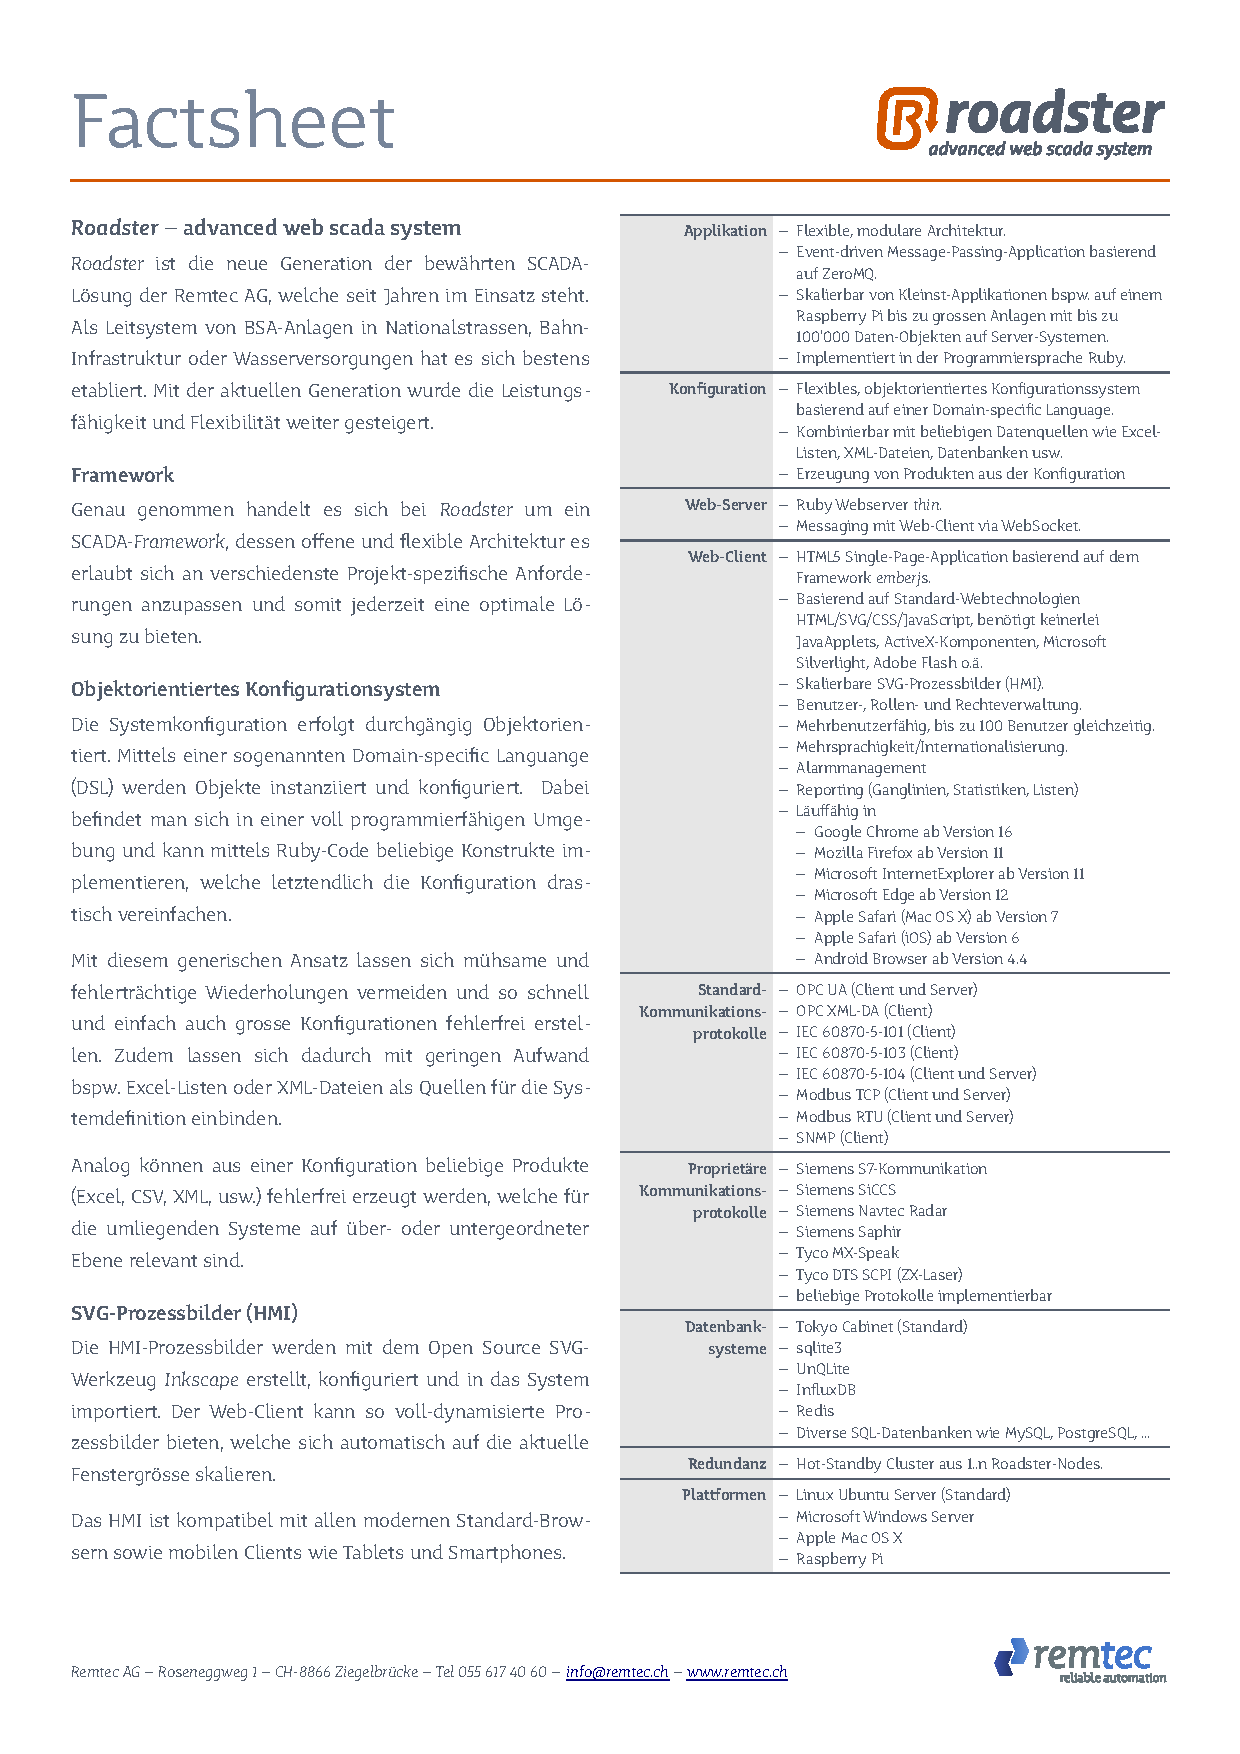
\includegraphics[trim=14.8cm 27cm 1cm 1.4cm, clip=true, width=0.38\textwidth]{img/roadster_factsheet.pdf}\end{raggedright}

\par\vspace{30mm}
{\scshape\Large Bachelor thesis\par}
\vspace{1.5cm}
{\huge\bfseries Roadster High Availability\par}
\vspace{2cm}
{\Large\itshape Manuel Schuler, Patrik Wenger\par}
\vfill
for industry client\par
mindclue GmbH
\vfill
supervised by\par
Prof. Farhad Mehta

\vfill

% Bottom of the page
{\large Fall semester 2016\par}
\end{titlepage}

%-----------------------------------------------------------------------------
\begin{abstract}
\setcounter{page}{1}
\pagenumbering{roman}

% Introduction
TODO introduction

% Approach and Technologies
TODO approach and technologies

% Result
TODO result

\end{abstract}

%-----------------------------------------------------------------------------
\tableofcontents
\listoffigures
\listoftables
\lstlistoflistings

%-----------------------------------------------------------------------------
\chapter{Scope}
\setcounter{page}{1}
\pagenumbering{arabic}
\setcounter{secnumdepth}{0} % avoid section numbering here

TODO what's this scope about

\section{Goals}
TODO mandatory goals

\section{Optional Goals}
TODO optional goals

%-----------------------------------------------------------------------------
\part{Management Summary}\label{part:mgmtsummary}
\setcounter{secnumdepth}{3} % reset to default

\section{Initial Situation}
TODO describe initial situation, not too technical

\section{Software Development Process}
TODO describe decision to use RUP/Scrum
TODO maybe describe what project management tools we'll be using

\section{Project Phases}
TODO describe this phase in retrospection

\subsection{Inception}
TODO describe this phase in retrospection

\subsection{Elaboration}
TODO describe this phase in retrospection

\subsection{Construction}
TODO describe this phase in retrospection

\subsection{Transition}
TODO describe this phase in retrospection

\section{Results}
TODO describe results

%-----------------------------------------------------------------------------
\part{Technical Report}
\chapter{Context}

\section{Initial Situation}
TODO What's Roadster and its goals

\section{Software Architecture}
TODO Roadster architecture\\

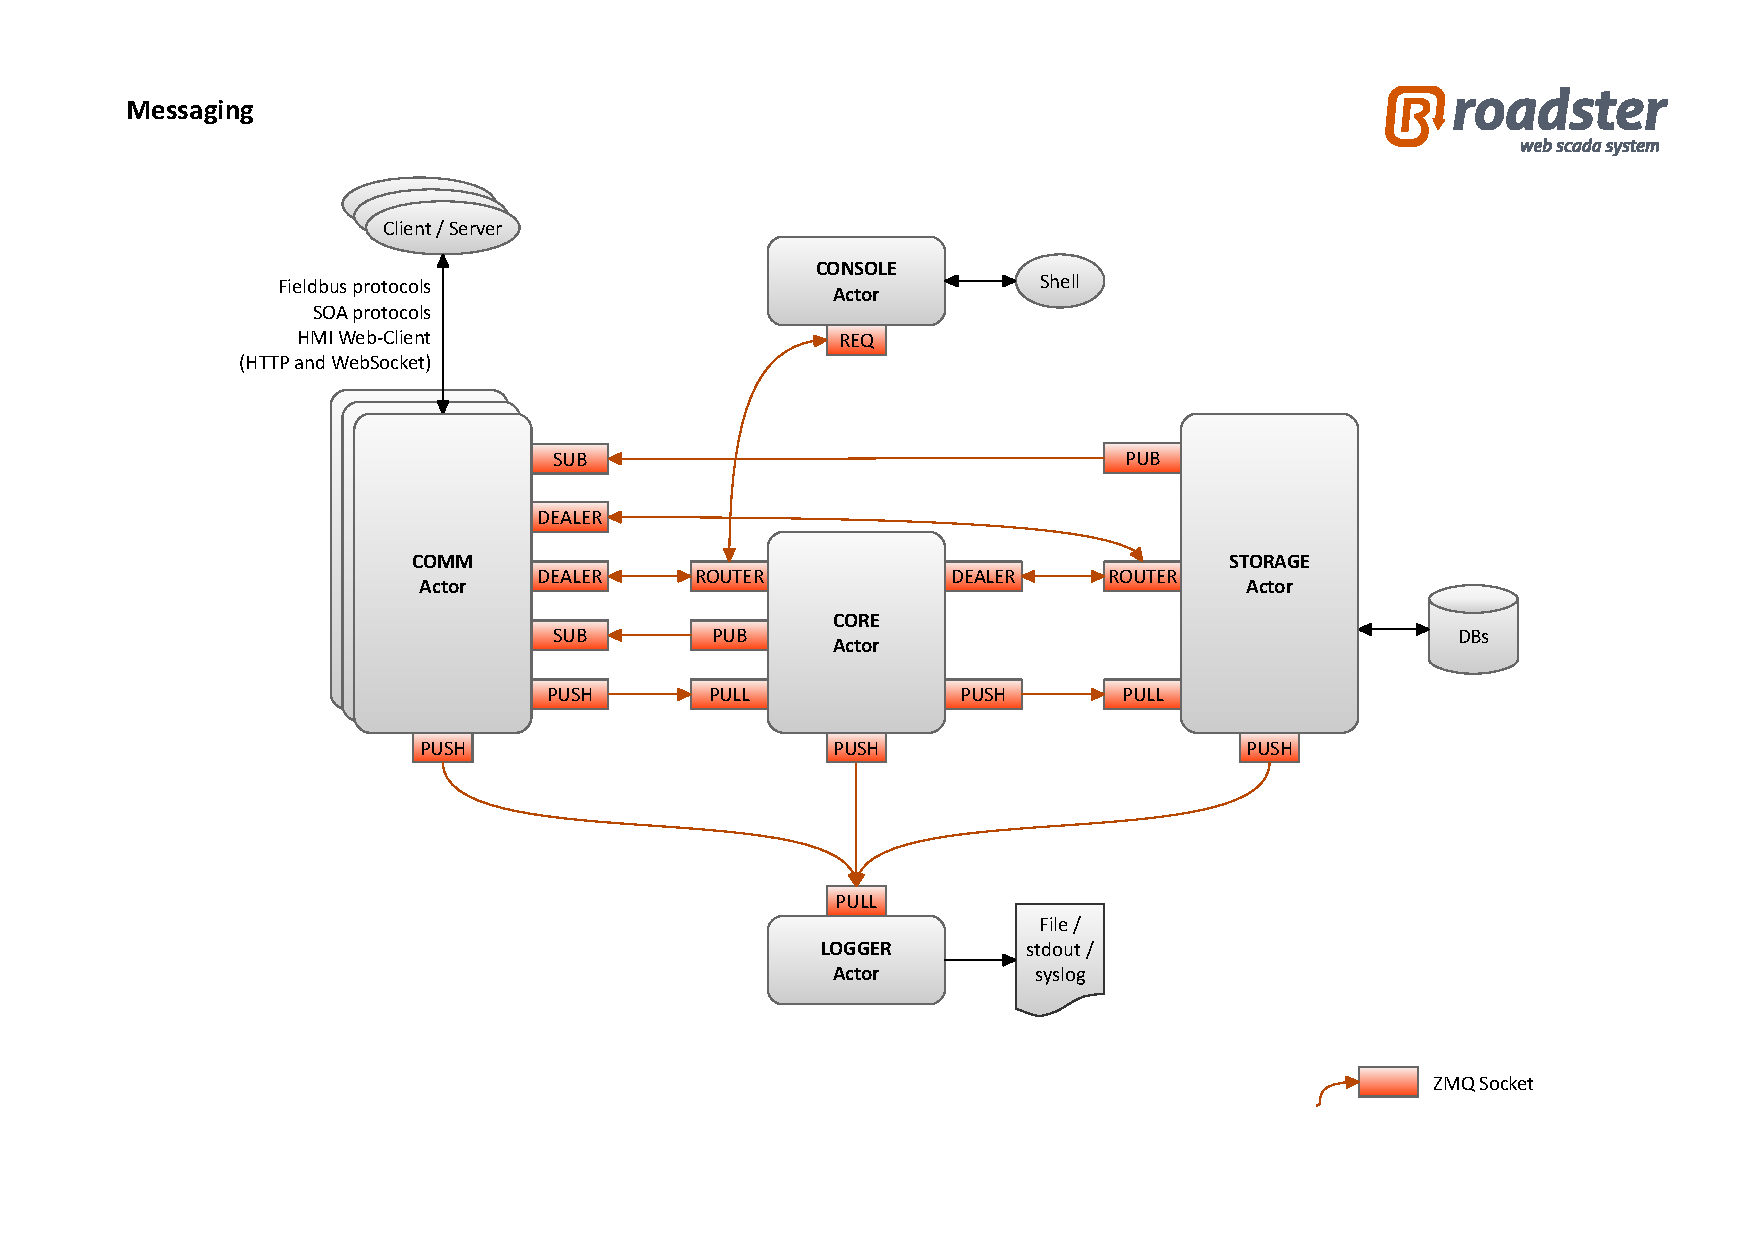
\includegraphics[trim=4cm 2cm 3.5cm 2.8cm, clip=true, width=\textwidth]{img/roadster_arch.pdf}

\section{Problem Description}

TODO our tasks

\subsection{Non-Functional Requirements}

TODO the NFRs

\chapter{About ZMQ}

TODO crash course in ZMQ/CZMQ/CZTop

\chapter{Port}\label{ch:port}
\section{Concept}
TODO explain concept

\chapter{Cluster}\label{ch:cluster}
TODO explain Clustered Hashmap Protocol (I guess)

\section{Implementation}
TODO explain how to implement/integrate CHP

\chapter{High Availability}\label{ch:ha}

\section{Concept}
TODO explain binary star pattern and how to implement/integrate it

\section{Implementation}
TODO explain how to implement/integrate Binary Star

\chapter{Optional Goal: Highly Available OPC UA Server}\label{ch:opc-ua-server}

TODO explain new opportunity for OPC UA HA server

\section{Concept}
TODO describe whatever needs to be described

\section{Implementation}
TODO describe whatever needs to be described

\chapter{Conclusion}
TODO write conclusion, we're the best and everything is awesome

\printbibliography

%-----------------------------------------------------------------------------
\appendix
\part{Appendix}
\chapter{Self Reflection}
TODO how did we perform, completion of goals, accuracy of estimated efforts, efficiency, resourcefulness

\section{Thank You}
TODO anyone we'd like to thank

\chapter{Formalities}
\section{Declaration of Originality}
We hereby confirm that we are the sole authors of this document and the
described changes to the Roadster framework and libraries developed.

TODO any usage agreements or license
%\includepdf[width=\textwidth,pages=1,pagecommand=\section{Permissions},trim=1.9cm 3cm 2cm 2cm,clip]{vereinbarung.pdf}

\chapter{Project Plan}

\section{Organization}
TODO roles, how we organize ourselves and how we communicate with each other

\chapter{Infrastructural Problems}\label{ch:problems}
TODO describe serious problems here, if any

TODO add any other appendix chapters here, like detailed ZMQ stuff, usage manuals, ...

\end{document}
